% 1977 年上海卷理科第 7 题：等腰梯形
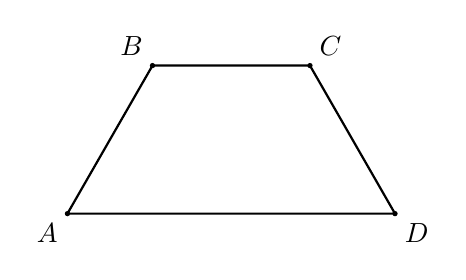
\begin{tikzpicture}[scale=0.8]
  \coordinate (A) at (0,0);
  \coordinate (D) at (5.2,0);
  \coordinate (B) at (1.35,2.35);
  \coordinate (C) at (3.85,2.35);
  \draw[thick] (A)--(B)--(C)--(D)--cycle;
  \fill (A) circle (1.2pt) node[below left] {$A$};
  \fill (B) circle (1.2pt) node[above left] {$B$};
  \fill (C) circle (1.2pt) node[above right] {$C$};
  \fill (D) circle (1.2pt) node[below right] {$D$};
\end{tikzpicture}
